\section{Approach Overview}
This section presents the high-level ideas behind both the pre-processing and on-the-fly synthesis techniques. The pre-processing aims to determine the synthesis result directly based on the input formula and the input/output pair. First of all, it is trivial to know that the formula cannot (resp. can) be realizable if it is unsatisfiable (resp. valid). Therefore, one can run the satisfiability checkers, such as \aaltaf\citep{LRPZV19}, to check the satisfiability of the input formula before synthesis, ruling out the meaningless instances (Theorem \ref{thm:sat-syn}). Next, for an \ltlf formula with the atomic set $\X\cup\Y$, if there is $Y\in 2^{\Y}$ such that $Y\models\phi$ is true ($Y$ is a length-one finite trace), we can know that $\phi$ is realizable (Theorem \ref{thm:winning-1}). Consider $\phi = \G (a\vee b)$ with $\X=\{a\}$ and $\Y=\{b\}$ as an example. Since $\{b\}\models\phi$ is true, $\phi$ is realizable. 
For an unrealizable formula $\phi$, we first define the \emph{projection} (Definition \ref{def:fp}), i.e., $\phi|_{P_{\phi}}$, which is a Boolean formula including all first-position elements of traces accepted by $\phi$. Then, if there is no $Y\in 2^{\Y}$ such that $Y\models\phi|_{P_{\phi}}$ is true, we can conclude that $\phi$ is unrealizable (Theorem \ref{thm:failure-1}). For instance, consider $\phi = \G (a\wedge b)$ with $\X=\{a\}$ and $\Y=\{b\}$. We can know $\phi$ is unrealizable even without constructing the corresponding \dfa. Finally, we introduce a stronger but easier-implementing version of Theorem \ref{thm:failure-1}, saying that if there exists $X\in 2^{\X}$ such that $X\models\phi|_{P_{\phi}}$ is not true, then $\phi$ is unrealizable (Theorem \ref{thm:failure-2}).  

We apply the \SAT-based technique in \cite{LRPZV19}, which constructs automata (\NFA) states on the fly for the \ltlf formula, to the synthesis problem. Given state $\phi$ (essentially a formula), the technique can generate a \emph{propositional assignment}, which includes one transition information starting from the state $\phi$. We adapt this technique accordingly such as to generate one transition for the transition-based \DFA (\tdfa, a variant of \dfa that is better for on-the-fly construction). Then, the new methodology creates \tdfa states in four different ways as shown in Figure \ref{fig:demonstration}. In the figure, from current state $s_1$, our approach creates state $s_2$ by fixing $Y_0\in 2^{\Y}$ and enumerating $X\in 2^{\X}$ (currently is $X_0$). After that,
\begin{itemize}
    \item[(a)]  if $s_2$ cannot be recognized as winning or failure, the DFS (Depth-first Search) strategy is applied to create a new state $s_3$;
    \item[(b)] if $s_2$ is recognized as winning, another $X\in 2^{\X}$ (here is $X_1$) is selected by fixing $Y_0$, obtaining a new state $s_3$. If all successor states are winning, then $s_1$ is winning;
    \item[(c)] if $s_2$ is recognized as failure, another $Y\in 2^{\X}$ (here is $Y_1$) is selected and $Y_0$ is ruled out from the winning strategy in current search. If no more $Y$ can be selected, $s_1$ is a failure state;
    \item[(d)] if $s_2$ has been visited before, i.e., a loop is found during the state computation, we can prove that choosing $Y_0$ cannot belong to the winning strategy in current search, and another $Y\in 2^{\X}$ (here is $Y_1$) has to be selected. 
\end{itemize}

One can see that our on-the-fly approach is able to return either realizable or unrealizable result before the whole \dfa is constructed. 

\begin{figure}
    \centering
    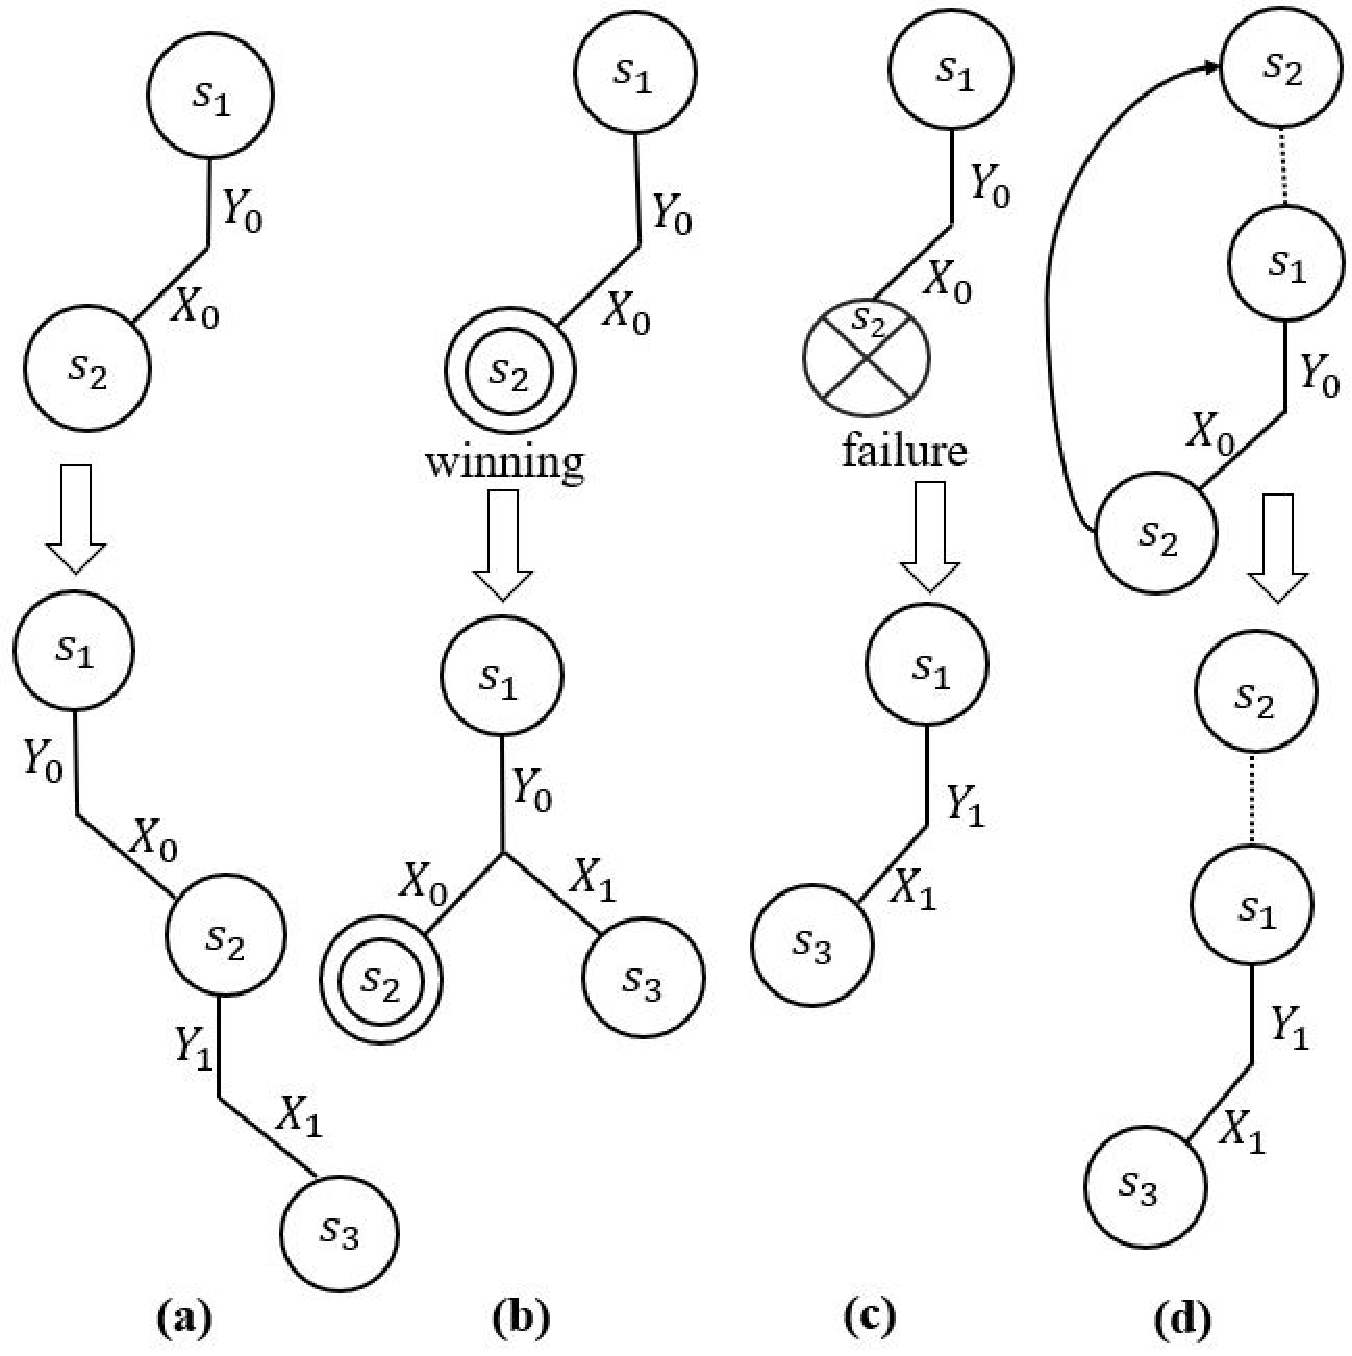
\includegraphics[scale=0.35]{demonstration.pdf}
    \caption{A demonstration of key operations for on-the-fly \ltlf synthesis.}
    \label{fig:demonstration}
\end{figure}



